% This must be in the first 5 lines to tell arXiv to use pdfLaTeX, which is strongly recommended.
%\pdfoutput=1
% In particular, the hyperref package requires pdfLaTeX in order to break URLs across lines.

%\documentclass[11pt]{article}

% Remove the "review" option to generate the final version.
%\usepackage[review]{acl}

% Standard package includes
%\usepackage{times}
%\usepackage{latexsym}

% For proper rendering and hyphenation of words containing Latin characters (including in bib files)
%\usepackage[T1]{fontenc}
% For Vietnamese characters
% \usepackage[T5]{fontenc}
% See https://www.latex-project.org/help/documentation/encguide.pdf for other character sets

% This assumes your files are encoded as UTF8
%\usepackage[utf8]{inputenc}

% This is not strictly necessary, and may be commented out,
% but it will improve the layout of the manuscript,
% and will typically save some space.
%\usepackage{microtype}
%\usepackage{url,color}
%\usepackage{amsmath}
%\usepackage{verbatim}
%\usepackage{booktabs}
%\usepackage{bm}
%\usepackage{graphicx}
%\usepackage{natbib}
%\usepackage{multirow,array}
%\usepackage{bbm}
%\usepackage{algorithm}
%\usepackage{algorithmic}
%\usepackage{xcolor}
%\usepackage{caption}
%\usepackage{amsfonts,amssymb} 
%\newcommand{\secref}[1]{Section \ref{#1}}
%\newcommand{\figref}[1]{Figure \ref{#1}}
%\newcommand{\eqnref}[1]{Eq. (\ref{#1})}
%\newcommand{\tabref}[1]{Table \ref{#1}}
%\newcommand{\exref}[1]{Example \ref{#1}}
%\newcommand{\KZ}[1]{\textcolor{blue}{Kenny: #1}}

%\begin{document}
	
	\appendix
	
	\begin{table*}[thb!]
		\centering
		\scriptsize
		\begin{tabular}{lccccc}
			\toprule
			Models & SST-2~(67K)                                                  & QQP~(364K)                                                    & QNLI~(105K)                                                   & MNLI-m/mm~(393K)                                                   & SQuAD v1.1~(88K)                                             \\
			\midrule
						Metric & Accuracy                                                  & Accuracy                                                    & Accuracy                                                   & Accuracy                                                   & F1 score                                            \\
						\midrule
			 Percent of \#Param.~$\downarrow$ &25\% ~16\%  ~~8\%            &25\% ~16\%  ~~8\%             &25\% ~16\%  ~~8\%            &25\% ~~~~~~~~~	~16\%  ~~~~~~~~~~8\%            &25\% ~16\%  ~~8\%            \\
			\midrule
		 \multicolumn{6}{c}{\textit{Task-agnostic Distillation}}   \\
			\midrule
			DistilBERT      & 88.9 ~86.4 ~83.0          & 89.4~ 88.0~ 82.4          & 83.8~ 81.6~ 64.9          &  76.4/76.4 ~71.6/70.9 ~59.8/58.6           & 78.0~ 66.5 ~28.5          \\
			PD-BERT         & 88.2~ 87.5~ 82.7          & 89.8 ~88.9 ~82.9          & 86.1~ 83.4~ 65.9          & 78.6/78.3 ~75.9/75.9 ~66.0/65.9          & 77.0 ~45.2~ 22.8          \\
			TinyBERT        & 89.8 ~88.0 ~82.6          & 90.0~ 88.7~ 83.2          & 87.7 ~84.5~ 63.1          & 80.6/80.5~ 77.1/77.7~ 65.6/66.2         & 58.0 ~38.1 ~15.4          \\
			\midrule
			 \multicolumn{6}{c}{\textit{Task-specific Distillation}}   \\
				\midrule
			BERT$_{\text{Truncated}}$ & 87.7 ~85.6 ~79.6          & 88.0~ 86.9 ~82.2          & 83.0 ~78.7 ~60.3          & 75.7/73.2~ 73.1/72.3~ 60.6/60.3          & 54.8~ 31.4~ 17.1          \\
			Vanilla KD         & 88.5~ 86.5 ~82.0           & 88.8~ 87.2 ~82.3          & 83.6 ~78.6~ 59.8          & 76.1/73.5 ~73.3/72.6~ 61.3/61.2          & 62.5 ~32.3~ 17.0          \\
			PKD        & 88.1~ 87.2 ~82.0          & 88.5~ 87.5 ~82.3          & 82.7~ 78.0~ 59.8          & 75.8/75.6 ~73.0/72.3~ 61.3/61.2          &60.5~ 31.5~ 17.0                                                      \\
			BERT-of-Theseus & 88.5~ 86.1~ 79.6          & 89.0 ~86.0 ~82.2          & 85.0 ~80.3~ 60.3          & 76.3/76.4~ 73.4/73.6 ~60.6/60.3         &72.7~ 63.2~ 26.2                                                      \\
			RAIL-KD        & 88.8~ 86.8~ 83.9          &90.2 ~88.6 ~83.3          &85.7 ~81.2~ 65.7          &78.8/78.8 ~73.5/74.0 ~62.1/61.4         &78.7~ 69.5~ 32.1                                                      \\
			CKD        & 89.8 ~88.7~ 84.1          & 90.1~ 88.9~ 82.9          & 87.0~ 84.9 ~67.6          & 79.1/78.9 ~76.8/76.8~ 66.4/66.7          &78.9~ 69.1~ 33.1                                                      \\
			MetaDistil         & 88.9 ~87.0~ 82.7          & 88.9~ 86.9~ 82.1          & 86.8~ 84.9 ~67.5          & 79.2/79.7 ~76.7/77.0~ 66.4/66.7          &78.8~ 69.0~ 32.4                                                      \\
			\midrule
			 \multicolumn{6}{c}{\textit{Model Architecture-dependent Structured Pruning}}   \\
			\midrule
			SP-$l_0$        & \underline{90.4} ~\underline{89.4}~ \underline{87.9}         & 90.1 ~89.3~ 85.5          & 88.7 ~87.2~ 84.9          & 81.9/82.5~ 80.8/81.2~ 76.2/77.0          &84.9~ 81.9~ 69.8          \\
			ISP        & 89.7 ~89.2~ 87.0         & 90.2 ~89.9~ \underline{89.0}          & 88.6 ~88.1~ 84.9          & 80.8/80.9~ 80.5/80.1~ 78.5/79.2          & 81.7~ 78.7~ 73.7          \\
			\midrule
		   \multicolumn{6}{c}{\textit{Matrix Factorization}}   \\
			\midrule
			SVD        & 88.9 ~88.1~ 84.5         & 90.0 ~87.9~ 83.1          & 86.1 ~83.8~ 67.6          & 79.6/80.2~ 76.6/76.7~ 71.6/72.2         & 85.5~ 81.1~ 51.3          \\
			LPAF-CAP~(ours)       &89.8 ~89.2~ 87.5 &\textbf{90.5} ~\textbf{90.4}~ \textbf{89.3}    &\underline{89.0}~ \underline{88.3}~ \underline{85.2}  &\underline{81.9}/\underline{82.6}~ \textbf{81.5/82.0}~ \textbf{79.5}/\underline{80.3}    &\underline{86.5}~ \underline{85.6}~ \underline{81.8}    \\
			LPAF-SMvP~(ours)       & \textbf{90.7~ 89.7~ 88.5} & \underline{90.4}~ \underline{90.1}~ \underline{89.0} & \textbf{89.2~ 88.6~ 85.7} & \textbf{82.2/82.9}~ \underline{81.4}/\underline{81.9}~ \underline{79.2}/\underline{80.1}& \textbf{87.2 ~85.7 ~82.0} \\
			\bottomrule
		\end{tabular}
		\caption{Experimental resutls of all compared BERT compression methods. The best results are \textbf{bolded} and the second best are \underline{underlined}. The numbers in the parenthesis are the size of training data for each task.}
		\label{table:all}
	\end{table*}
	
	\begin{table}[h!]
		\centering
		\footnotesize
		\begin{tabular}{l|l|lll}
			\toprule
			\multicolumn{2}{c|}{Model}                          & SST-2       & QNLI          & QQP           \\
			\midrule
			\multicolumn{2}{l|}{POMP-100}  &87.50       & 84.72     &89.11        \\
			\multicolumn{2}{l|}{POMP-80}  &86.12       &83.07      &88.32        \\
			\multicolumn{2}{l|}{POMP-60}  &85.89       &80.29      &87.16        \\
			\multicolumn{2}{l|}{POMP-40}  &84.29       &70.49      &83.47        \\
			\bottomrule
		\end{tabular}
		\caption{Experimental results of low-rank factoriztion upon models produced by post-training one-shot magnitude pruning~(POMP).}
		\label{table:pomp}
	\end{table}
	
	\begin{table}[h!]
		\centering
		\footnotesize
		\begin{tabular}{l|l|lll}
			\toprule
			\multicolumn{2}{c|}{Model}                          & SST-2       & QNLI          & QQP           \\
			\midrule
			\multicolumn{2}{l|}{LTH-100}  &87.50       &84.50      &89.10        \\
			\multicolumn{2}{l|}{LTH-80}  &86.70       &83.86      &88.46        \\
			\multicolumn{2}{l|}{LTH-60}  &85.00       &79.81      &87.54        \\
			\multicolumn{2}{l|}{LTH-40}  &85.67       &68.00      &85.77        \\
			\bottomrule
		\end{tabular}
		\caption{Experimental results of low-rank factoriztion upon models produced by the lottery ticket hypothesis~(LTH).}
		\label{table:lth}
	\end{table}
	
	\section{Distributions of Rank}
	\label{sec:appendixA}
	
	
	\begin{figure}[h]
		\centering
		\scalebox{0.54}{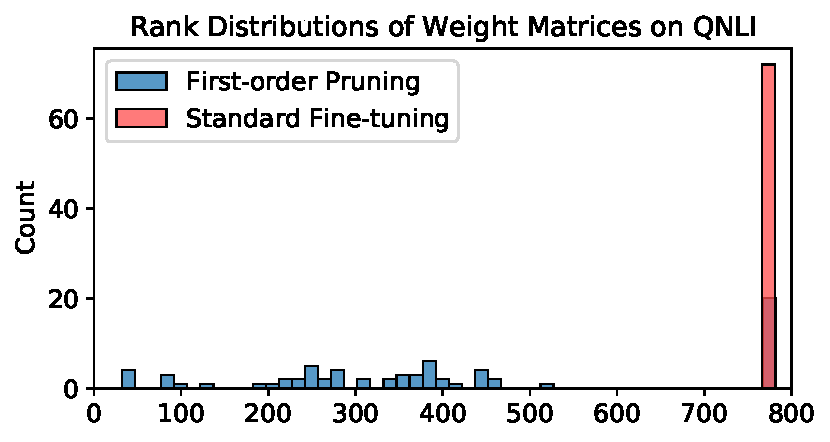
\includegraphics{./figures/rank_dist.pdf}}
		\caption{The rank distribution of weight matrices of models trained by standard fine-tuning and first-order pruning~(SMvP). For zero-order pruning~(both post-training one-shot magnitude pruning and Lottery Ticket Hypothesis), we observe a similar distribution as standard fine-tuning, hence we do not show it in the figure.}
		\label{fig:rank}
	\end{figure}
	As described in the pilot experiment, the average rank of models produced by first-order pruning algorithms is much lower than that of models produced by standard fine-tuning and zero-order pruning algorithms. Concretely, we show the respective rank distribution on QNLI dataset in \figref{fig:rank}. As can be observed, for first-order pruning,  a large portion of ranks are distributed at 100-200. In stark contrast, the densely fine-tuned model is nearly full-rank. This phenomenon highlights the possibility of effective model compression using low-rank factorization on models produced by first-order pruning algorithms.
	
	
	
	
	\section{Low-rank Factorization on Zero-order Pruning Algorithms}
	\label{sec:appendixB}
	
	
	In the paper, we primarily adopt soft-movement pruning~(SMvP) as our default choice of first-order pruning algorithm. To give more clear evidence of how the rank-distribution of a model affects the downstream performance after factorization, we also present the results of post-training one-shot magnitude pruning~(POMP) and lottery ticket hypothesis~(LTH) in \tabref{table:pomp} and \tabref{table:lth}. Compared to Table 1 in Section 3, we can see that the downstream performance of low-rank factorization upon models produced by zero-order pruning algorithms is on par with that of SVD while being much lower than our proposed LPAF, verifying the necessity of a low-rank structure for low-rank factorization to retain satisfactory task performance.
	
	
	\section{Detailed Results of Compared Compression Methods}
	\label{sec:appendixC}
	
	
	We present the detailed experimental results of all compared BERT compression methods in \tabref{table:all}. All these methods are able to offer a perceivable reduction in memory and computation without resorting to specialized linear algebra implementation or hardware. We can categorize these methods into four types: 
	\begin{itemize}
		\item Task-agnostic distillation methods, which include DistilBERT, PD-BERT, and TinyBERT. They realize different levels of compression rate by varying the number of encoder layers.
		\item Task-specific distillation methods, which include baselines in the second part of \tabref{table:all}. They realize different levels of compression rate by varying the number of encoder layers They also differ from how the student model is initialized: PKD initializes the student model with the lowest fewer layers from the teacher model; RAIL-KD leverage DistilBERT as initialization for distillation, which naturally provides a 
		better starting point. CKD instead uses PD-BERT as initialization, which is also proven to be more effective  than the strategy of PKD.
		\item We also include the results of  Iterative Structured Pruning~(\textbf{ISP}) which progressively removes attention heads in multi-head attention layer and neurons in the feed-forward layer with the lowest importance scores. The importance score of a specific structure $s$ is measured by the expected gradient of the loss function $\mathcal{L}$ with respect to the mask variable $\epsilon_s$ associated with it:
		\begin{align}
			I_s = \mathbb{E}_{x\sim \mathbb{X}}|\frac{\partial \mathcal{L}(x)}{\partial \epsilon_s}|
		\end{align}
		ISP achieves BERT compression by locally slimming specific structures without explicitly reducing number of encoder layers. Different from ISP that reach target compression rate in an iterative manner, we experiment with structured pruning with $l_0$ regularization that explicitly control the compression rate by modifying the  training objective, denoted as \textbf{SP-$l_0$}. SP-$l_0$ draws samples from the hard-concrete distribution as approximation to binary masks for different structures.
		
		Note that we omit ISP and SP-$l_0$ in the main experiment because they are both model architecture-dependent and require troublesome re-organization of different model structures to realize perceptible memory and computation reduction. In contrast, LPAF performs \textit{inerratic} matrix decomposition, making efficient inference straightforward.
				\item Factorization-based methods including SVD and our LPAF that shrink the original model without changing the number of layers.
	\end{itemize}
	
	Although many task-specific compression methods like BERT-of-Theseus have demonstrated improvement over task-agnostic methods like TinyBERT under conventional compression setting~(e.g., compressing a 12-layer teacher model into a 6-layer student model), they actually perform worse under relatively high compression ratio, i.e., $\ge4.0$x. The reason might be that under a high compression regime, pure task-specific compression without utilizing the pre-compression stage has limited generalization ability due to: 1) insufficient network capacity. 2) ineffective knowledge transfer from the teacher because of the large capacity gap in between.
%\end{document}

